\section{Experiments}

\subsection{Memory-side Bottlenecks}

Figure~\ref{fig:l2drambandwidth} shows the memory bandwidth observed from DRAM and L2 cache in an
NVIDIA GTX 680 GPU when memory accesses are not coalesced. To see how much more memory bandwidth
adding each SM can consume from DRAM or L2, we varied the number of thread blocks (each containing
1024 threads) from 1 to 8 so that we can implicitly vary the number of utilized SMs (our GPU has 8
SMs). To calculate the memory bandwidths, two synthetic benchmarks are used in which threads of each
warp access non-coalesced locations of memory.\footnote{To make threads access non-coalesced
locations of memory, threads in a warp access data in disjoint 128-byte regions.} The only
difference between the two benchmarks is that in the first one, all accesses are to DRAM while in
the second one all accesses are serviced by the L2 cache. To access data in DRAM each thread is
programmed to access data items with 32-bytes strides in between so that none of the accesses are
hits in the L2 (the L2 cache-line size is 32-bytes). To access data in L2, each thread is
programmed to first fill in the cache, and then perform memory loads that would map to the existing
cache-lines.

\begin{figure}[t]
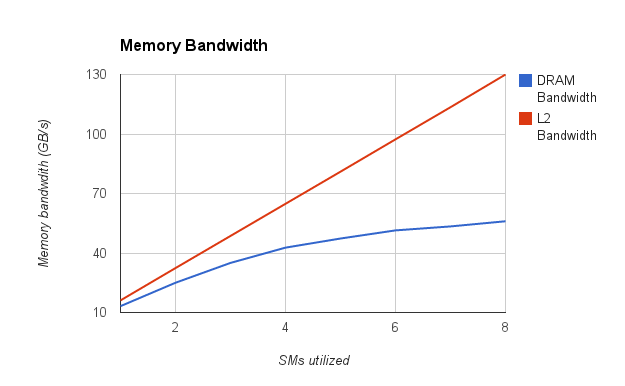
\includegraphics[scale=0.35]{DRAML2bandwidth.png}
\caption{DRAM and L2 memory bandwidths.}
\label{fig:l2drambandwidth}
\end{figure}


As depicted, by increasing the number of SMs, memory bandwidths observed from DRAM and L2 are both
increased. Note that, increase in the number of SMs practically represents the increase in the
number of memory request bus lanes which in turn, represents the increase in the number of memory
requests that can be carried by those lanes. The increase in L2 memory bandwidth is quite linear
while the increase in DRAM memory bandwidth diminishes substantially as more SMs are utilized.
However, regardless of how well each one of them scale with more number of SMs, it appears that both
DRAM and L2 cache can potentially service more memory requests from possibly more number of SM --
i.e. the bandwidth lines are not flat at the end of the graph).

 
We argue that, the two lines in Figure~\ref{fig:l2drambandwidth} show lower and upper bounds for
memory bandwidth of applications that access memory in a non-coalesced fashion. In other words, the
memory bandwidth of such application hardly gets lower than the DRAM line, and also rarely gets
higher than the line that represents the L2 memory bandwidth.\footnote{A few rare scenarios exist in
which bandwidth could become worse than DRAM line or better than L2 line. For example, if accesses
to DRAM results in an unusual rate of GPU memory bank conflict, the bandwidth might further drop, or
if some accesses are cached by L1 or constant caches, the bandwidth might be higher than the L2
line.} This means that the memory bandwidth of these applications typically lies somewhere between
the two lines and thus, is limited not because DRAM+L2 are exhausted, but because memory request bus
cannot service more memory requests.


\subsection{L1 Cache Behavior}

Our experience with GPUs indicate that traditional L1 caches might not be suitable for modern GPUs.
This is in part because of the small size of L1 caches and in part due to the massively parallel
nature of GPU execution model which is quite distinct from that of traditional CPU. In GPU execution
model, thousands of GPU threads share the same L1 cache, frequently context switching on the shared
computing cores. Therefore, most of the data that is loaded into the cache will be evicted before
that data is accessed again. Therefore, the L1 cache hit rate is typically so low that it might not
be worth it to add the circuitry of caching and lookup in the critical path of every memory access.
As a result, L1 caches often degrade performance instead of improving it, as also observed by
others~\cite{jia2012characterizing}.

\begin{figure}[t]
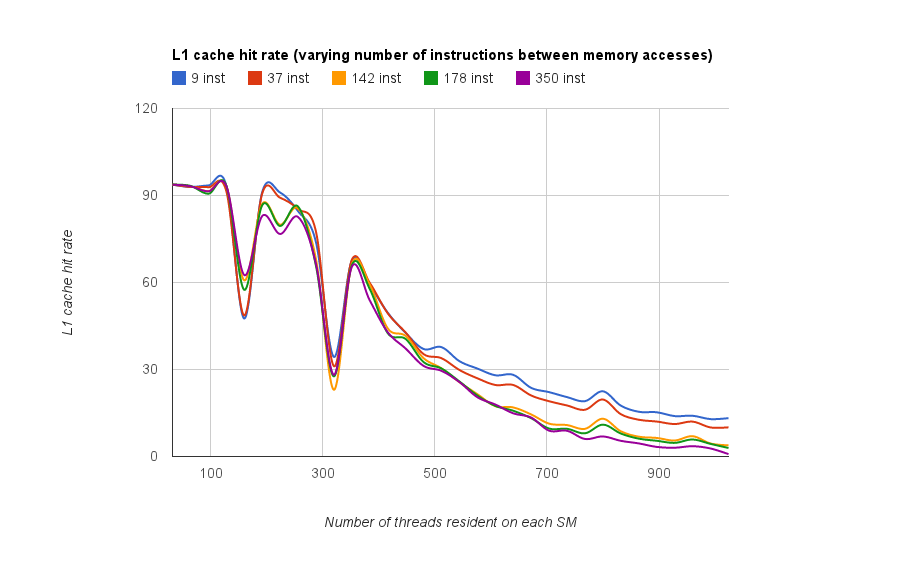
\includegraphics[scale=0.35]{l1SingleAccess.png}
\caption{L1 cache hit rate. Single access in a loop.}
\label{fig:l1single}
\end{figure}


Figure~\ref{fig:l1single} shows the L1 cache hit rate of a simple synthetic benchmark in which each
thread sums up elements of a different chunk of an array in a loop. We utilized only one SM by
issuing only one thread block, and only varied the number of threads in that block. The benchmark
should ideally receive high cache hit rate as each thread accesses adjacent locations of memory in
the loop and therefore, exhibits high spatial locality. However, the hit rate drops way before the
parallelism reaches a point where most applications typically need to achieve a reasonably good
computational performance.

To better show the behavior of L1 caches in real-world applications, we injected some pure
arithmetic instructions in the body of the loop. These instructions would impose some delay between
subsequent memory accesses that each thread makes in the subsequent loop iterations. Noticeably,
cache hit rate further drops as more instructions are executed between memory accesses\footnote{The
number of instructions shows the number of {\it machine} instructions.}

%There's a very interesting trade-off: more threads are required to utilize GPU memory. less threads
%are required to not thrash the cache...

\begin{figure}[t]
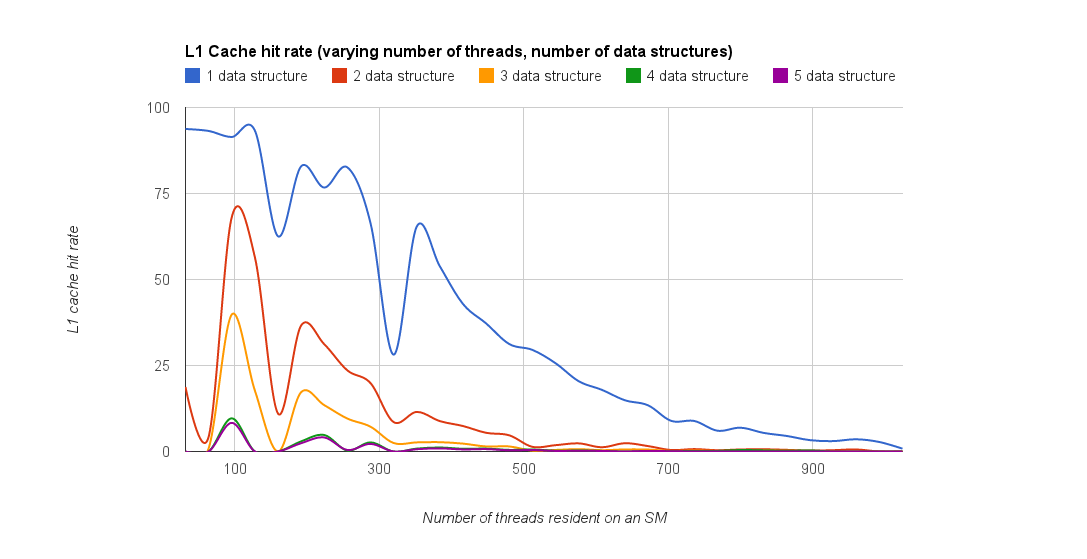
\includegraphics[scale=0.25]{l1MultipleAccess.png}
\caption{L1 cache hit rate. Multiple accesses in a loop.}
\label{fig:l1multiple}
\end{figure}


Figure~\ref{fig:l1multiple} shows the cache hit rate of the same benchmark, when threads are
accessing more than one array in the body of the loop. Similar to the first array, additional arrays
are also partitioned into chunks, where each chunk is iterated on by a different thread, and
therefore, accesses to each array exhibit spatial locality. As depicted, adding even one more memory
access to a different array reduces the L1 cache hit rate dramatically. When accessing two arrays,
the cache hit rate degrades to less than 5\% when running 512 threads. Given that in modern
architectures, SMs can host up to 2048 running threads, issuing 512 threads only achieves 25\%
thread occupancy in SMs, which is considered to be low provided the guidelines of GPU programming
best practices.

%Obviously, it might be seen as a trade-off between the number of threads and the cache hit rate.
%But, as we will show in our experiments in section X, this trade-off is hardly a win for the cache.

